\section{Algoritmo de Previsão de Stocks}\label{sec34}

Uma vez que para uma boa gestão de stocks existe a necessidade de prever a duração de cada um dos itens em stock, com base no historial de consumo e reposição da casa. De forma a garantir este requisito inerente ao sistema Smart Stocks, implementou-se um algoritmo de previsão de stocks.

Para a realização deste algoritmo, foram analisados os vários tipos de modelo existentes e adotar o mais adequado ao sistema. Durante a pesquisa, deparou-se com a existência de dois tipos de modelo de previsão, sendo eles, Modelos Quantitativos e Qualitativos \cite{GestaoStocks:MetodosPrevisaoStocks}. Os primeiros baseiam-se em análises numéricas dos dados históricos, enquanto que os qualitativos privilegiam dados subjetivos baseados na opinião de especialistas. Como se deseja realizar este algoritmo com base no histórico de consumo e reposição, optou-se pelo Modelo Quantitativo. 

Dos sub-modelos disponíveis elegeu-se um modelo de séries temporais visto que este pode incluir nos seus dados um conjunto de elementos, por exemplo, sazonalidade, tendências, influências cíclicas ou comportamento aleatório. Decidiu-se, então, utilizar o método da média móvel devido a esta ser simples e fácil de implementar e ser suficiente para o desenvolvimento do projeto. No entanto, dentro do método da média móvel existem diversos tipos, dos quais escolheu-se o da média móvel ponderada, que é uma variação do modelo da média móvel simples em que os valores dos períodos mais recentes recebem um peso maior que os valores correspondentes aos períodos anteriores, podendo assim dar maior relevância aos dados mais atuais.

%
% Implementação
%
\subsection{Implementação}\label{subsec341}

Aplicou-se o método da média móvel ponderada para um período mínimo de 3 semanas. Este procedimento começa por atribuir pesos aos dados consoante a semana a que se referem, sendo que as mais recentes têm maior peso.

Como se tratam de dados diários, e de forma a evitar a descompensação de valores provocada por dias com consumo excecionais, amortecem-se  os valores. Assim os resultados tornam-se mais homogéneos e com um comportamento mais sazonal.   

Com base nestes dois aspetos construiu-se um dia comum numa casa, que servirá de base para uma previsão. Seguiu-se o seguinte procedimento:


\textbf{1º Passo}\\
A primeira fase consiste em aplicar o método da média móvel ponderada aos dados, para isso usou-se a seguinte expressão:

\begin{equation} 
Pdiax'= T1 \times Rdia1 + T2 \times Rdia2 + T3 \times Rdia3
\end{equation}

Onde os valores de $Tx$ correspondem às taxas definidas como pesos para os dados diários ($Rdiax$) da semana $x$, sendo a semana mais recente a com o valor superior. As taxas escolhidas foram: 
\begin{center}
	\textit{T1 = 10\%, T2 = 30\% e T3 = 60\%}
\end{center}
A escolha destes valores foi realizada de modo a atribuir determinados pesos a cada elemento, garantindo que a soma de todos os pesos seja igual a 100\%, tendo em atenção em dar um peso maior às semanas mais recentes. Testou-se a equação com diferentes valores, sempre com a mesma ideia de definir pesos maiores para as semana mais recentes, não observando alterações significativas.\\

\textbf{2º Passo}\\
Aos valores obtidos anteriormente aplicou-se um método de amortização de forma a homogeneizar e harmonizar a previsão. Assim, o valor obtido para um dia da semana resulta da soma do seu valor e do valor do dia da semana anterior e da seguinte, multiplicados por taxas, ou seja: 

\begin{equation} 
Pdiax''= Tant \times PdiaxAnt' + Tdiax \times Pdiax' + Tseg \times PdiaxSeg'
\end{equation}

Onde os valores de $Tant$, $Tdiax$ e $Tseg$ correspondem às taxas definidas como pesos para os dias da semana anterior, atual e seguinte, respetivamente. Os valores $PdiaxAnt'$, $Pdiax'$ e $PdiaxSeg'$ são os valores previstos no 1º passo do método de previsão para os dias da semana anterior, atual e seguinte, respetivamente. As taxas escolhidas foram: 

\begin{center}
	\textit{Tant = Tseg = 25\%  e Tdiax = 50\%.}
\end{center}
A escolha destes valores foi realizada de modo a atribuir determinados pesos a cada elemento, garantindo que a soma de todos os pesos seja igual a 100\%, tendo em atenção dar um peso maior ao dia da semana a calcular. Testou-se a equação com diferentes valores, sempre com a mesma ideia de definir um peso maior ao dia da semana a calcular, não observando alterações significativas, como se pode observar no gráfico seguinte.

%T1=0.1 T2=0.3 T3=0.6
%Tant=0.25 Tdia=0.5 Tseg=0.25

%T1=0.1 T2=0.3 T3=0.6
%Tant=0.2 Tdia=0.5 Tseg=0.3

%T1=0.1 T2=0.3 T3=0.6
%Tant=0.3 Tdia=0.5 Tseg=0.2

\begin{center}
    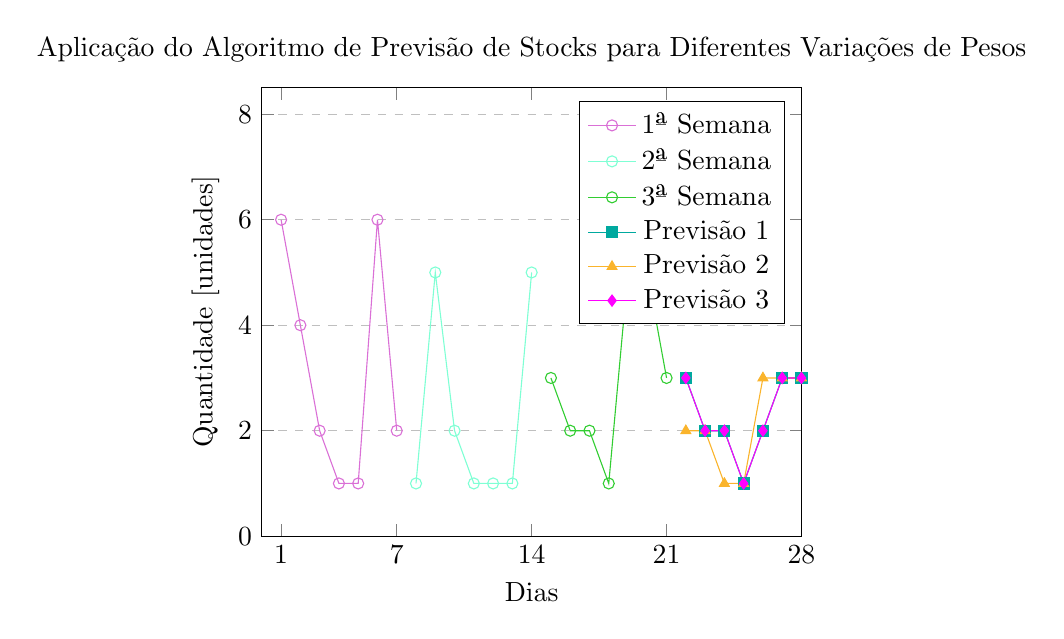
\begin{tikzpicture}
        \begin{axis}[
            title={Aplicação do Algoritmo de Previsão de Stocks para Diferentes Variações de Pesos},
            xlabel={Dias},
            ylabel={Quantidade [unidades]},
            xmin=0, xmax=28,
            ymin=0, ymax=8.5,
            xtick={1, 7, 14, 21, 28},
            ytick={},
            legend pos=north east,
            ymajorgrids=true,
            grid style=dashed,
        ]
        \addplot[
            color=Orchid,
            mark=o,
            ]
            coordinates {
            (1,6)(2,4)(3,2)(4,1)(5,1)(6,6)(7,2)
            };
            
        \addplot[
            color=Aquamarine,
            mark=o,
            ]
            coordinates {
            (8,1)(9,5)(10,2)(11,1)(12,1)(13,1)(14,5)
            };
            
        \addplot[
            color=LimeGreen,
            mark=o,
            ]
            coordinates {
            (15,3)(16,2)(17,2)(18,1)(19,5)(20,5)(21,3)
            };
            
        \addplot[
            color=Emerald,
            mark=square*,
            ]
            coordinates {
            (22,3)(23,2)(24,2)(25,1)(26,2)(27,3)(28,3)
            };
            
        \addplot[
            color=Dandelion,
            mark=triangle*,
            ]
            coordinates {
            (22,2)(23,2)(24,1)(25,1)(26,3)(27,3)(28,3)
            };
        
        \addplot[
            color=Magenta,
            mark=diamond*,
            ]
            coordinates {
            (22,3)(23,2)(24,2)(25,1)(26,2)(27,3)(28,3)
            };
        \legend{1ª Semana,2ª Semana,3ª Semana,Previsão 1, Previsão 2,Previsão 3}
        \end{axis}
    \end{tikzpicture}
\end{center}




A Previsão 1 foi calculada com os pesos Tant = Tseg = 25\% e Tdia = 50\%. A Previsão 2 com os pesos Tant = 20\%, Tdia = 50\% e Tseg = 30\%.
E a Previsão 3 com Tant = 30\%, Tdia = 50\% e Tseg = 20\%.

%
% Integração
%
\subsection{Integração no Sistema Smart Stocks}\label{subsec342}

De forma a tornar o sistema Smart Stocks independente de um só algoritmo de previsão de stocks, estipulou-se uma interface para separar o contrato da implementação. De forma geral, a informação mínima exigida a cada dia para se obter a previsão de uma semana é: o nome do produto, a sua quantidade e a respetiva data do dia em questão. Esta informação compõe um objeto, que pode ser utilizado pelas várias implementações do algoritmo de previsão de stocks.

Foi criada uma \textit{task}, a ser executada periodicamente \footnote{Para efeitos de teste, a periodicidade da \textit{task} é de 5 minutos. No entanto, num cenário real esta tarefa seria executada no final de cada dia.}, cuja função é percorrer todos os itens na base de dados, obter o seu histórico de quantidades e realizar a previsão para a semana seguinte. De seguida, os dados obtidos da previsão são analisados, e caso a quantidade prevista esteja abaixo de um determinado limite \footnote{Considera-se como stock mínimo de segurança, a quantidade mínima abaixo da qual um produto é inserido na lista de compras. Atualmente, esse limite está definido como duas unidades de um item em stock (\acrshort{sku}). No entanto, este é um ponto a melhorar. Esta melhoria poderia consistir no utilizador poder definir os seus próprios valores limite,  através de configurações nas aplicações cliente.}, este item é inserido na lista de compras gerida pelo sistema Smart Stocks. 
